\documentclass{beamer}

\usepackage[polish]{babel}
\usepackage[utf8]{inputenc}
\usepackage[T1]{fontenc}
\usepackage{dirtytalk}
\usepackage{microtype}
\usepackage{luavlna}
\DeclareRobustCommand{\stirling}{\genfrac\{\}{0pt}{}}
\binoppenalty=10000
\relpenalty=10000
\setlength{\emergencystretch}{3em}

\usetheme{Madrid}

\title{Modularity i jego modyfikacje w rodzinach grafów gęstych}
\author{Zofia Kuriata}
\institute{Politechnika Wrocławska}
\date{28 stycznia 2026}

\begin{document}

\begin{frame}
    \titlepage
\end{frame}

\begin{frame}{Modularity}
    \begin{block}{Modularity}
        Miara jakości podziału grafu na społeczności.
    \end{block}
    \vspace{0.5cm}
    \begin{block}{Definicja}
        \(G\) graf z co najmniej jedną krawędzią, \(\mathcal{A}\) partycja zbioru wierzchołków \(G\).\\
        \vspace{0.4cm}
        Modularity score \(\mathcal{A}\) wynosi \(mod_{\mathcal{A}}(G) = \sum_{A \in \mathcal{A}} \left(\frac{e(A)}{e(G)} - {\left(\frac{vol(A)}{vol(G)}\right)}^2\right).\)\\
        \vspace{0.4cm}
        Modularity grafu \(G\) wynosi \(mod(G) = \max_{\mathcal{A} \in \mathcal{P}(V)} mod_{\mathcal{A}}(G).\)
    \end{block}

\end{frame}

\begin{frame}{Modularity}
    \begin{block}{Zastosowanie}
        \begin{itemize}
            \item Analiza sieci społecznych, biologicznych, informatycznych.
            \item Algorytmy klasteryzacji Louvain, Leiden.\\
        \end{itemize}

    \end{block}
    \vspace{0.2cm}
    \begin{block}{Wady}
        \begin{itemize}
            \item \textit{Resolution limit} - pomijanie małych społeczności w dużych grafach.
            \item Ignorowanie wewnętrznej struktury społeczności.
            \item Nienaturalnie duże wartości.\\
        \end{itemize}
    \end{block}
\end{frame}

\begin{frame}{Modularity star}
    \begin{block}{Modularity star}
        Zmodyfikowana wersja modularity eliminująca niektóre wady klasycznej wersji.\\
    \end{block}
    \vspace{0.5cm}
    \begin{block}{Definicja}
        \(G\) graf z co najmniej jedną krawędzią, \(\mathcal{A}\) partycja zbioru wierzchołków \(G\).\\
        \vspace{0.4cm}
        Modularity star score \(\mathcal{A}\) wynosi \(mod^*_{\mathcal{A}}(G) = \sum_{A \in \mathcal{A}} \left(\frac{e(A)}{e(G)} - {\left(\frac{vol(A)}{vol(G)}\right)}^2\right) \cdot \left(\frac{\Delta(A) + 1}{|A|}\right)\), gdzie \(\Delta(A)\) to maksymalny wewnętrzny stopień wierzchołka w społeczności \(A\).\\
        \vspace{0.4cm}
        Modularity star grafu \(G\) wynosi \(mod^*(G) = \max_{\mathcal{A} \in \mathcal{P}(V)} mod^*_{\mathcal{A}}(G).\)
    \end{block}

\end{frame}

\begin{frame}{Cel}
    W literaturze większość badań dotyczy grafów rzadkich, ja natomiast skupiłam się na \textbf{grafach gęstych}.\\
    \vspace{0.2cm}
    \begin{block}{Cele pracy}
        \begin{itemize}
            \item Własności: modularity \(\rightarrow\) na modularity star.
            \item Ograniczenie górne na modularity star.
            \item Liczba krawędzi do usunięcia z \(K_n\), aby \(mod^* > 0\).
            \item Hipotetyczna odpowiedź na pytanie czy istnieje \(G\), dla którego \(mod^*(G) > mod(G)\).
        \end{itemize}
    \end{block}
\end{frame}

\begin{frame}{Zachowane własności}
    \(G\) graf z co najmniej jedną krawędzią, \(\mathcal{A}\) partycja zbioru wierzchołków \(G\).\\
    \vspace{0.2cm}
    W pracy wykazałam, że następujące własności modularity przenoszą się na modularity star.
    \vspace{0.2cm}
    \begin{itemize}
        \item \(-\frac{1}{2} \leq mod_{\mathcal{A}}^*(G) < 1\).
        \item Jeśli \(|\mathcal{A}|\leq 2\)  oraz \(\displaystyle \max_{\mathcal{B}: |\mathcal{B}| \leq 2} (mod_{\mathcal{B}}^*(G)) = mod_{\mathcal{A}}^*(G)\), to
              \[\forall_{A \in \mathcal{A}} \hspace{1mm} mod_A^*(G) \geq 0 .\]
        \item Jeśli \(mod_{\mathcal{A}}^*(G) = mod^*(G)\), to \(\mathcal{A}\) nie zawiera społeczności składającej się z pojedynczego wierzchołka stopnia 1.
        \item \((mod(G) = 0) \Leftrightarrow (mod^*(G) = 0)\).
    \end{itemize}
\end{frame}

\begin{frame}{Górne ograniczenie na modularity star}
    W pracy zaproponowałam następujące ograniczenie górne na modularity star
    \begin{block}{Twierdzenie}
        Dla grafu \(G=(V,E)\), gdzie \(|V|=n\):
        \[ mod^*(G) \leq \frac{n^2}{2} \cdot \max_{\mathcal{B}:|\mathcal{B}|\leq 2} mod_{\mathcal{B}}^*(G) \]
    \end{block}
    \vspace{0.5cm}
    \begin{block}{Wniosek}
        Pozwala ono na ograniczenie wartości modularity star grafu poprzez przejrzenie jedynie partycji co najwyżej dwuelementowych. Jest szczególnie użyteczne w celu sprawdzenia czy modularity star danego grafu jest dodatnie.
    \end{block}

\end{frame}

\begin{frame}{Grafy prawie pełne}

    \begin{block}{Graf pełny \(K_n\)}
        \begin{itemize}
            \item dla \(n \geq 1\) mamy \(mod(K_n) = 0\) oraz \(mod^*(K_n) = 0\),
            \item dla \(n \geq 4\) istnieje graf \(G\) o \(n\) wierzchołkach, dla którego \(mod(G) > 0\) oraz \(mod^*(G) > 0\).\\
        \end{itemize}
    \end{block}

    \vspace{0.5cm}
    \textbf{Funkcja \(f^*(n)\):} Minimalna liczba krawędzi do usunięcia z \(K_n\), aby uzyskać \(mod^*(G) > 0\).

    \begin{alertblock}{Wynik}
        Dla każdej liczby naturalnej \(n \geq 4\):
        \[ f^*(n) = \left\lfloor\frac{n}{2}\right\rfloor + 1. \]
    \end{alertblock}
\end{frame}

\begin{frame}{Grafy prawie pełne dwudzielne}
    \begin{block}{Graf pełny dwudzielny \(K_{s,t}\)}
        Dla \(s,t \geq 1\):
        \[ mod(K_{s,t}) = 0 \quad \text{oraz} \quad mod^*(K_{s,t}) = 0 \]
    \end{block}

    \vspace{0.5cm}
    \textbf{Oznaczenie \(\delta^{-}_*(G)\):} Minimalna liczba krawędzi do usunięcia z \(G\), aby \(mod^*(G') > 0\).

    \begin{alertblock}{Wynik}
        Dla \(s,t \geq 1\):
        \[ \delta^{-}_*(K_{s,t}) = 1 \]
    \end{alertblock}
\end{frame}

\begin{frame}{Hipoteza 1: Ujemna kontrybucja}
    Jeśli \(mod_{\mathcal{A}}^*(G) = mod^*(G)\), to możliwe jest istnienie społeczności w \(\mathcal{A}\), która \textbf{kontrybuuje ujemnie} do mod star.
    \begin{figure}[H]
        \centering
        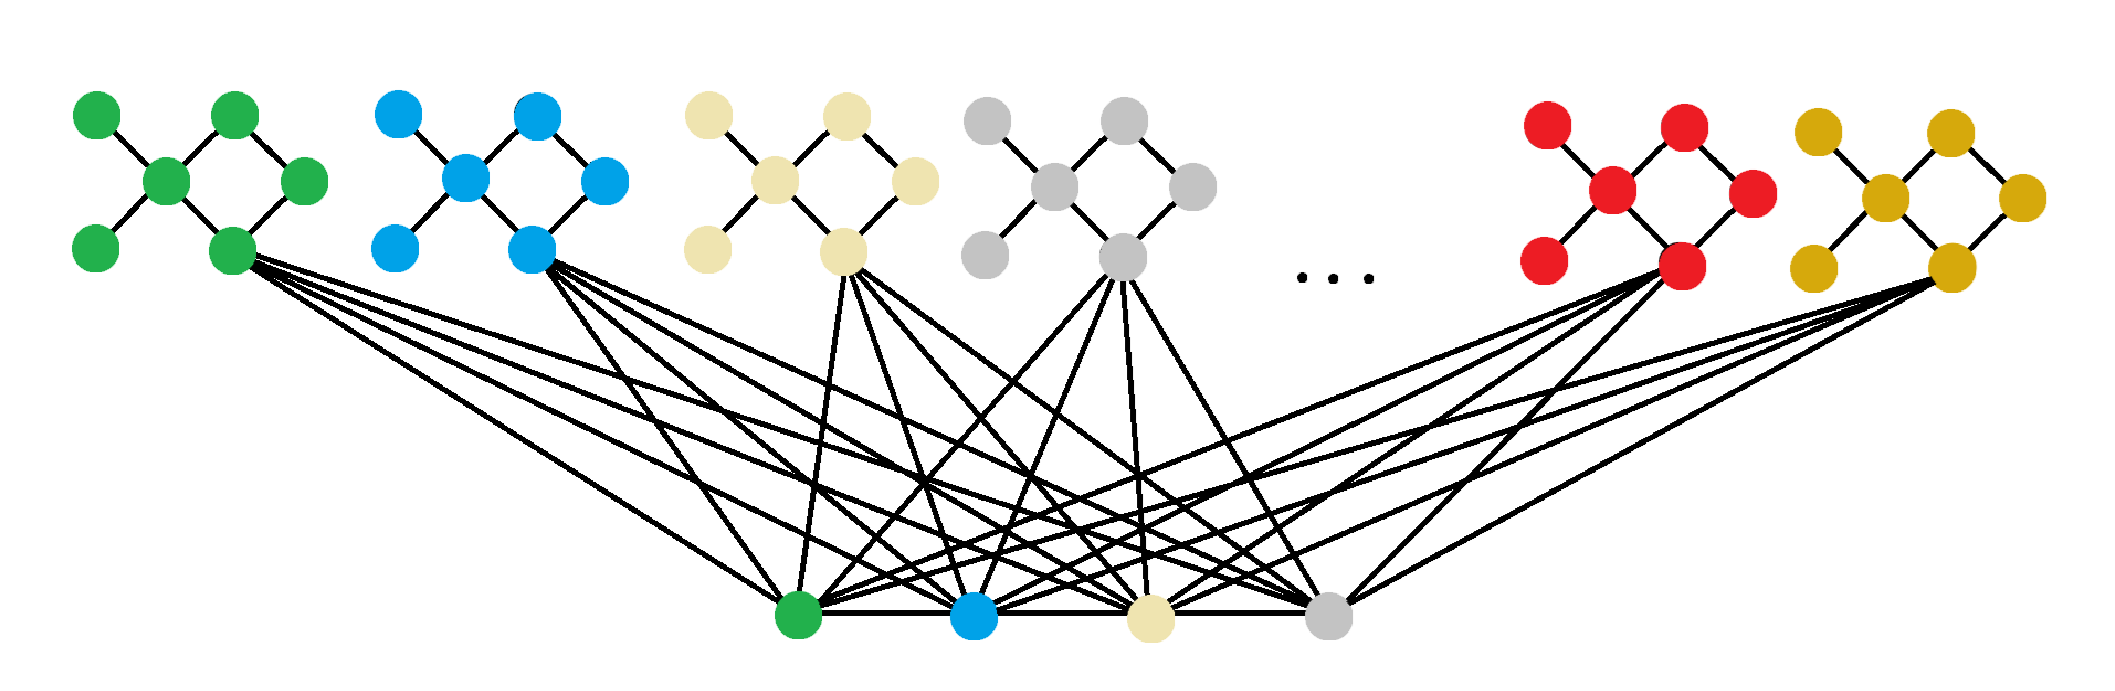
\includegraphics[width=0.8\textwidth]{../graphs/minus_mod.png}
        \caption{Ilustracja hipotezy.}
        \label{fig:thesis_mod_star}
    \end{figure}
    Wnioski:
    \begin{itemize}
        \item Dodawanie izolowanych wierzchołków wpływa na \(mod^*\).
        \item Społeczności w optymalnej partycji nie muszą indukować spójnych podgrafów.
    \end{itemize}
\end{frame}

\begin{frame}{Hipoteza 2: \(mod^* > mod\)}
    Istnieje graf \(G\), dla którego \(mod^*(G) > mod(G)\).
    \begin{figure}[H]
        \centering
        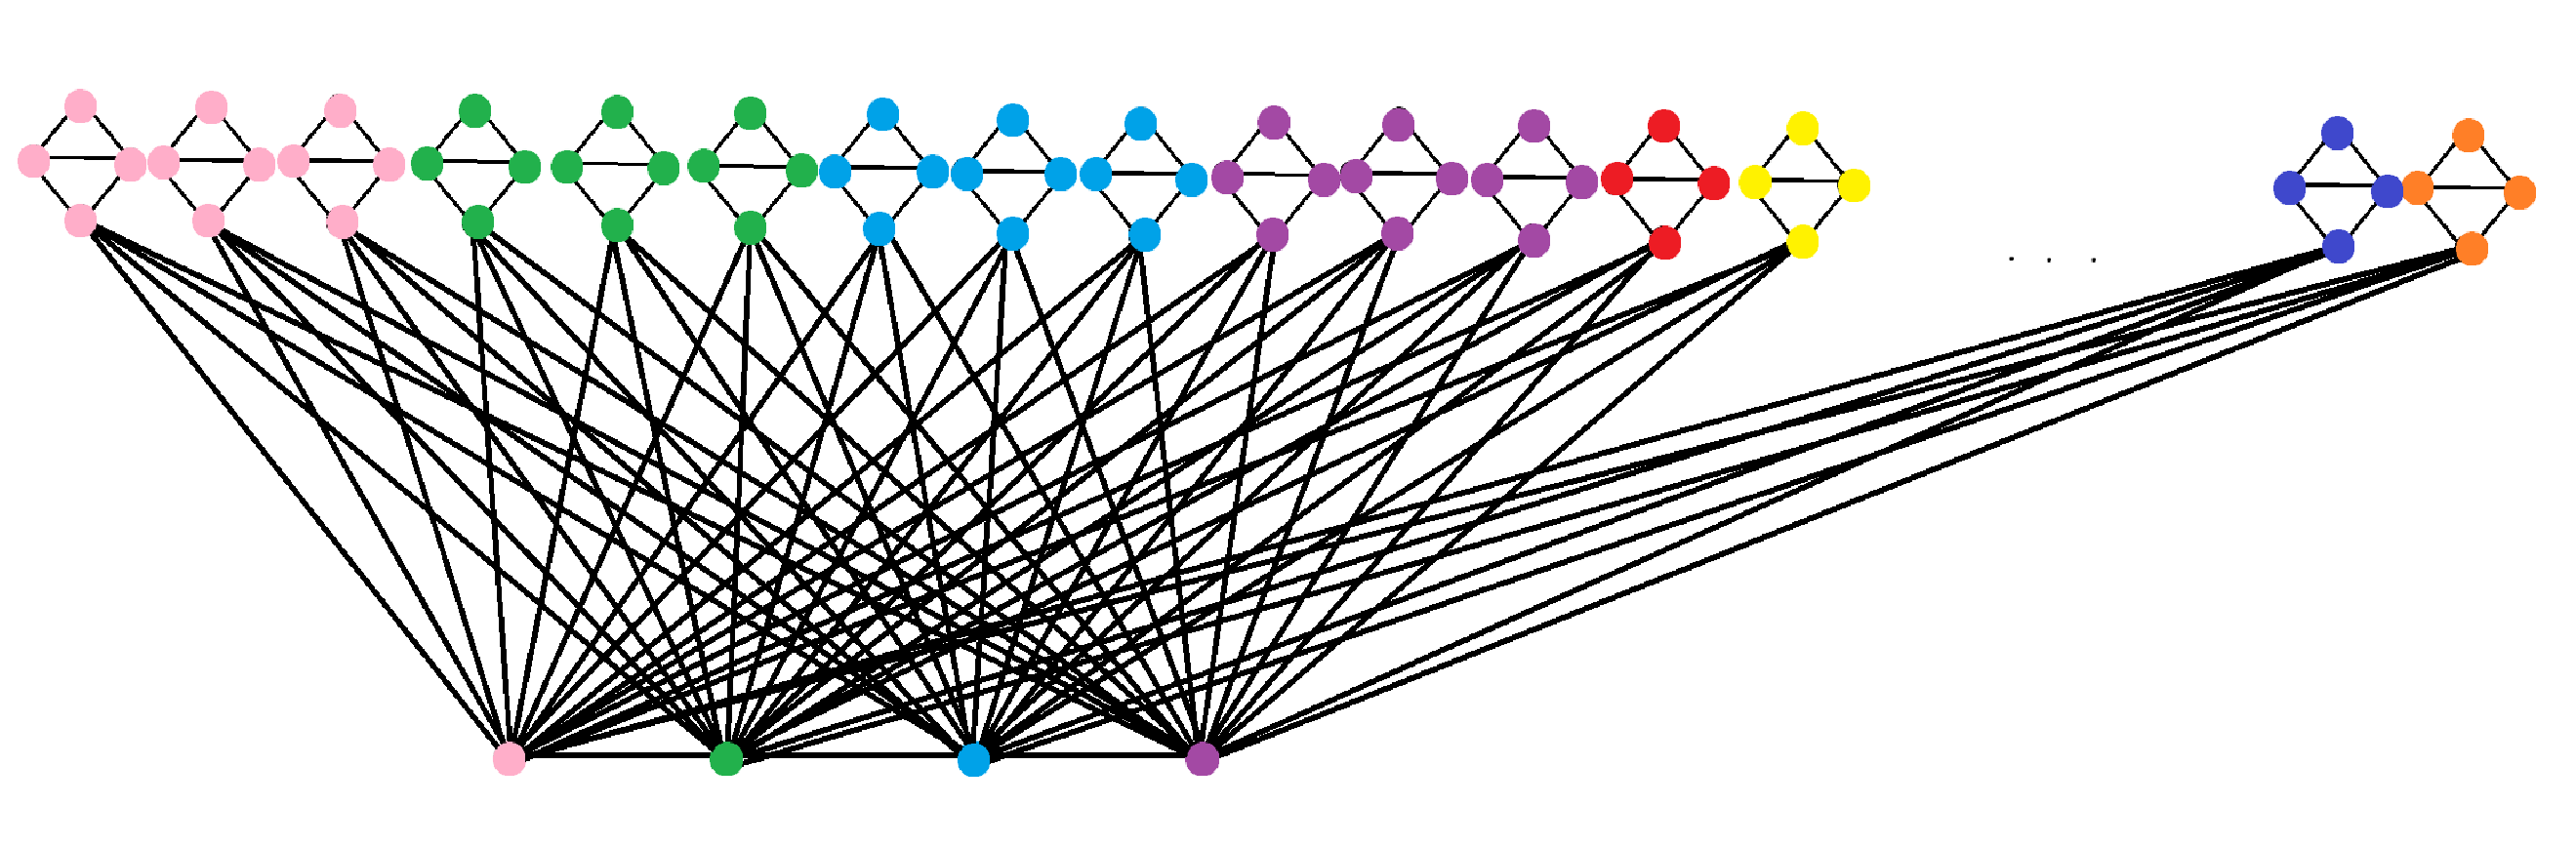
\includegraphics[width=0.9\textwidth]{../graphs/mod_star.png}
        \caption{Graf \(G\), dla którego hipotetycznie \(mod^*(G) > mod(G)\).}
        \label{mod_star}
    \end{figure}
    Największa znaleziona wartość \(mod^*_{\mathcal{A}}(G) \approx 0.5511554446\).\\
    \vspace{0.2cm}
    Największa znaleziona wartość \(mod_{\mathcal{A}}(G) \approx 0.54413127767\).
\end{frame}

\begin{frame}{Poszukiwania}
    Proces, który doprowadził do znalezienia \(G\):
    \begin{enumerate}
        \item Wyznaczenie warunków koniecznych, aby możliwe było spełnienie nierówności.
        \item Stworzenie modelu garfu spełniającego te warunki.
        \item Eksperymentalne dobranie parametrów.
        \item Testowanie sensownych partycji zbioru jego wierzchołków.
    \end{enumerate}
    \vspace{0.5cm}
    \begin{block}{Warunki konieczne}
        \begin{itemize}
            \item Najlepsze partycjonowanie dla mod i mod star muszą być różne.
            \item W optymalnym partycjonowaniu dla mod star musi istnieć \(\geq 1\) społeczność kontrybuująca ujemnie.
            \item Graf musi zawierać \say{rzadką} strukturę oraz pewną liczbę odpowiednio \say{gęstych} struktur.
        \end{itemize}
    \end{block}
\end{frame}


\begin{frame}{Algorytm Louvain}
    Algorytm Louvain służy do wykrywania społeczności w dużych grafach poprzez maksymalizację modularity score.
    \begin{columns}[T]
        \begin{column}{0.5\textwidth}
            \begin{enumerate}
                \item \textbf{Lokalna optymalizacja mod score}
                      \begin{itemize}
                          \item Każdy węzeł to osobna społeczność.
                          \item Przenosimy węzeł do sąsiada tylko, jeśli \textbf{zwiększa to mod score}.
                          \item Powtarzamy do osiągnięcia lokalnego maksimum.
                      \end{itemize}

                \item \textbf{Budowa meta-grafu}
                      \begin{itemize}
                          \item Społeczności stają się nowymi węzłami.
                          \item Krawędzie są sumowane.
                      \end{itemize}
            \end{enumerate}
            \small \textit{Proces iteruje, dopóki mod score może rosnąć.}
        \end{column}
        \begin{column}{0.5\textwidth}
            \begin{figure}[H]
                \centering
                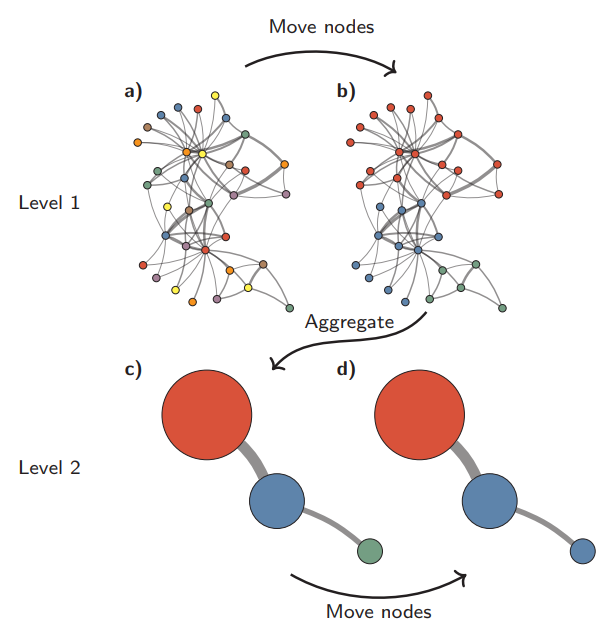
\includegraphics[width=0.9\textwidth]{../graphs/louvain.png}
                \caption{Algorytm Louvain \cite{TWE19}.}
                \label{louvain}
            \end{figure}
        \end{column}
    \end{columns}
\end{frame}

\begin{frame}{Algorytm Leiden}
    Ulepszona wersja alogrytmu Louvain. Rozwiązuje problem \textbf{niespójnych społeczności} oraz \textbf{resolution limit}. Wprowadza 3. fazę mającą na celu korektę nowopowstałego podziału na społeczności w fazie 1.
    \begin{enumerate}
        \item \textbf{Lokalna optymalizacja}.
        \item \textbf{Refinement}.
        \item \textbf{Agregacja}.
    \end{enumerate}
    \centering
    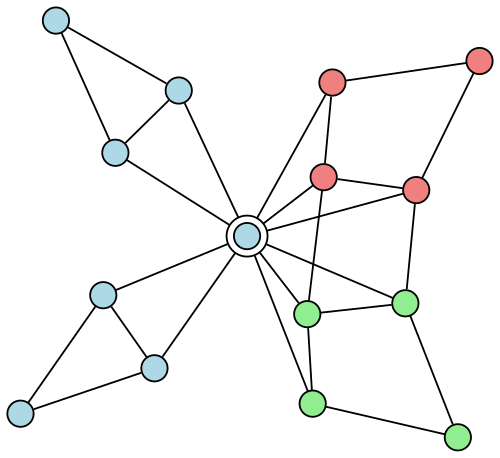
\includegraphics[width=0.3\textwidth]{../graphs/leiden1.png} \hfill
    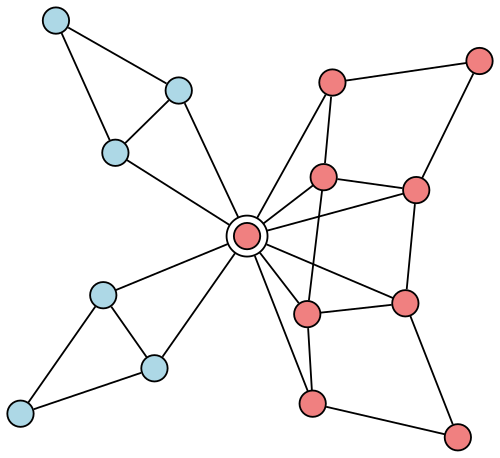
\includegraphics[width=0.3\textwidth]{../graphs/leiden2.png} \hfill
    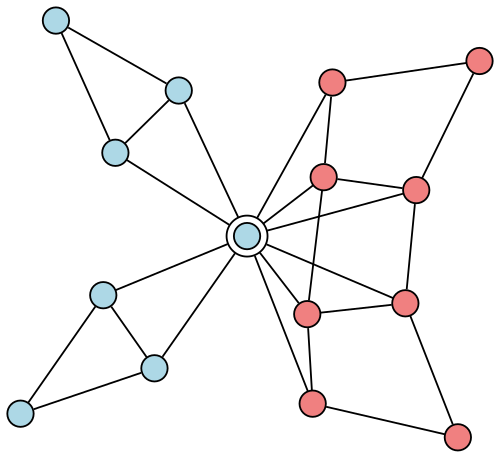
\includegraphics[width=0.3\textwidth]{../graphs/leiden3.png}
    \vfill
    {\tiny \url{https://en.wikipedia.org/wiki/Leiden_algorithm}}
\end{frame}

\begin{frame}{Złożoność obliczeniowa}
    Problem decyzyjny wyznaczenia modularity jest \textbf{NP-zupełny}.
    \vspace{0.5cm}
    \begin{block}{Przynależność do klasy NP}
        Dla danej partycji $\mathcal{A}$ i progu $k$, warunek $mod_{\mathcal{A}}(G) \geq k$ weryfikujemy w czasie wielomianowym.
    \end{block}

    \begin{block}{NP-trudność}
        Istnieje redukcja z silnie NP-zupełnego problemu \textbf{3-partition} do problemu modularity \cite{BD08}.
    \end{block}
\end{frame}

\begin{frame}{Redukcja}
    Dla instancji 3-partition $A = \{a_1, \ldots, a_{3k}\}$ budujemy graf $G(A)$ oraz wyznaczamy próg \(K(A)\).
    \vspace{0.5cm}
    \begin{columns}[T]
        \begin{column}{0.5\textwidth}
            \textbf{Struktura grafu:}
            \begin{itemize}
                \item $k$ klik o rozmiarze $a = \sum_{i=1}^{3k} a_i$.
                \item Dla każdego $a_i$ wierzchołek dodatkowy $v_i$.
                \item $v_i$ połączony z $a_i$ wierzchołkami \textbf{każdej} kliki.
            \end{itemize}
        \end{column}
        \begin{column}{0.5\textwidth}
            \textbf{Stopnie wierzchołków:}
            \begin{itemize}
                \item Węzeł kliki: $a$.
                \item Węzeł $v_i$: $k \cdot a_i$.
                \item Suma stopni: $2m = k \cdot a^2 + k \cdot a$.
            \end{itemize}
        \end{column}
    \end{columns}

    \vspace{0.5cm}
    W optymalnej partycji \(\mathcal{A}\) każda społeczność składa się z dokładnie \(1\) kliki i pewnej liczby dodatkowych wierzchołków \(v_i\).
\end{frame}

\begin{frame}{Redukcja}
    Mamy
    \begin{itemize}
        \item \(mod_{\mathcal{A}}(G(A)) = EC_{\mathcal{A}} - DT_{\mathcal{A}},\)
        \item \(EC_{\mathcal{A}}(G(A)) = \frac{m - (k-1)a}{m} = 1 - \frac{2k-2}{k(a+1)},\)
        \item \(DT_{\mathcal{A}}(G(A)) = \frac{1}{k^2a^2(a+1)^2} \cdot \sum_{A \in \mathcal{A}}vol(A)^2.\)
    \end{itemize}

    \begin{block}{Maksymalizacja modularity score}
        \(DT_{\mathcal{A}}(G(A))\) osiąga minimum równe \(\frac{k(a^2+a)^2}{k^2a^2(a+1)^2}\), gdy sumy stopni dodatkowych wierzchołków w każdej z $k$ społeczności są równe i wynoszą \(k \cdot \frac{1}{k} \cdot a = a\). Odpowiada to idealnemu podziałowi zbioru $A$ na podzbiory o sumie \(b = \frac{1}{k} \cdot a\).
    \end{block}
    \begin{alertblock}{Wyznaczenie progu}
        \[K(A) = 1 - \frac{2k-2}{k(a+1)}-\frac{ka^2(a+1)^2}{k^2a^2(a+1)^2} = \frac{(k-1)(a-1)}{k(a+1)}\]
    \end{alertblock}
\end{frame}

\begin{frame}{Poprawność redukcji}
    \vspace{1cm}
    \centering
    {\Large Istnienie 3-partycji dla zbioru $A$}

    \vspace{0.5cm}
    {\huge $\iff$}

    \vspace{0.5cm}
    \centering
    {\Large $mod(G(A)) \geq \frac{(k-1)(a-1)}{k(a+1)}$}
\end{frame}

\begin{frame}
    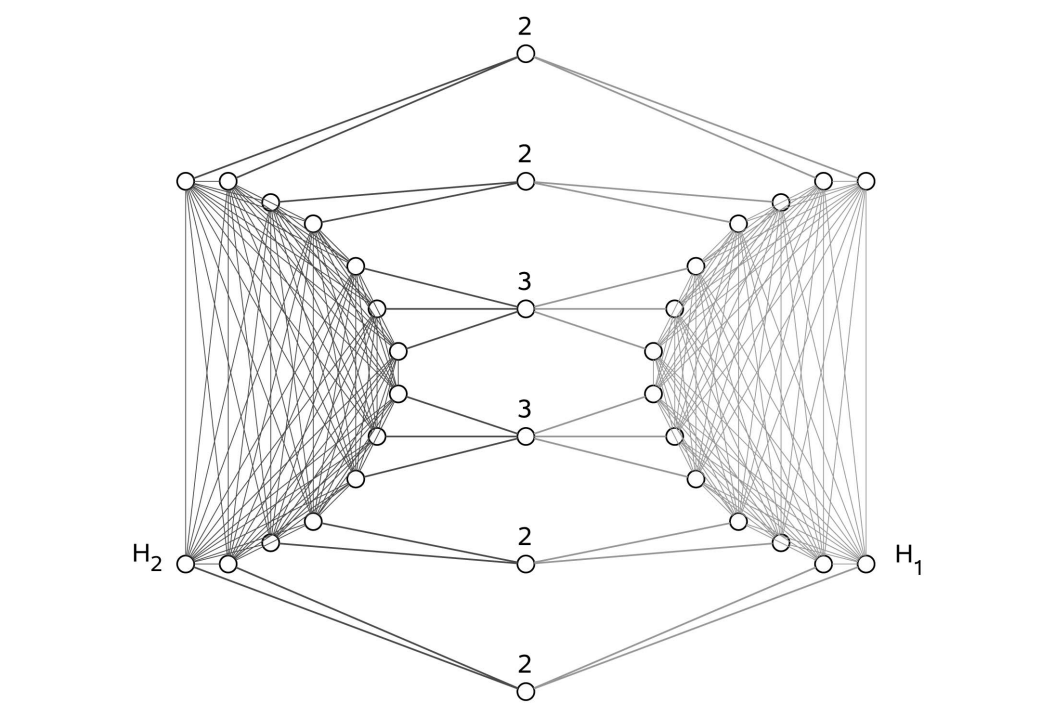
\includegraphics[width=1\textwidth]{../graphs/3partition.png}\hfill
    \cite{BD08}
\end{frame}

\begin{frame}{Liczby Bella}
    \begin{columns}
        \begin{column}{0.6\textwidth}
            \textbf{Definicja:} \(B_n\) to liczba wszystkich możliwych partycji zbioru n-elementowego.

            \[ B_n = \sum_{k=0}^{n}\stirling{n}{k} \]

            \textbf{Rekurencja:}
            \[ B_{n+1} = \sum_{k=0}^{n} \binom{n}{k} B_k.\]

            Tempo wzrostu: \(a^n < B_n < n!.\)
        \end{column}
        \begin{column}{0.4\textwidth}
            \centering
            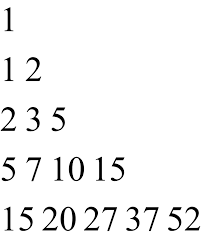
\includegraphics[width=0.9\textwidth]{../graphs/bell_triangle.png}
        \end{column}
    \end{columns}
\end{frame}

\begin{frame}{Liniowe równanie diofantyczne: $at - bs = 1$}

    Zakładamy, że \(\text{NWD}(t, s) = 1\).

    \vfill

    \begin{itemize}
        \item \textbf{Rozwiązanie szczególne:} Wyznaczamy $(a, b)$ za pomocą Rozszerzonego Algorytmu Euklidesa tak, aby \( at - bs = 1 \).

        \item \textbf{Rozwiązanie ogólne:} Wszystkie pary $(a', b')$ spełniające równanie dane są wzorami:
              \[
                  \begin{cases}
                      a' = a + s \cdot k \\
                      b' = b + t \cdot k
                  \end{cases} \quad \text{dla } k \in \mathbb{Z}.
              \]
              \(a't-b's = (a+s\cdot k)t - (b+t\cdot k)s = at-bs + skt - tks = 1\)
    \end{itemize}
\end{frame}

\begin{frame}{Rozszerzony Algorytm Euklidesa}
    \begin{block}{Cel algorytmu}
        Wyznaczenie współczynników całkowitych $a$ i $b$ takich, że:
        \[ at + bs = \text{NWD}(t, s) \]
    \end{block}

    \textbf{Procedura krok po kroku:}
    \begin{enumerate}
        \item \textbf{Algorytm Euklidesa:} Wykonujemy dzielenia z resztą, aż otrzymamy resztę $0$.
        \item \textbf{Wyznaczenie reszt:} Zapisujemy każde z powyższych równań w postaci: \textit{reszta = dzielna - iloraz $\cdot$ dzielnik}.
        \item \textbf{Podstawianie wsteczne:} Zaczynamy od równania z ostatnią niezerową resztą (NWD) i sukcesywnie podstawiamy poprzednie reszty, aż uzyskamy kombinację liczb $t$ i $s$.
    \end{enumerate}
\end{frame}

\begin{frame}{Przykład}
    \begin{exampleblock}{Przykład: $120a - 23b = 1$}
        \begin{itemize}
            \item \(120 = 5\cdot 23 + 5 \implies 5 = 120 - 5 \cdot 23\)
            \item \(23 = 4 \cdot 5 + 3 \implies 3 = 23 - 4 \cdot 5\)
            \item \(5 = 1 \cdot 3 + 2 \implies 2 = 5 - 1 \cdot 3\)
            \item \(3 = 1 \cdot 2 + 1 \implies 1 = 3 - 1 \cdot 2\)
        \end{itemize}
        \textbf{Wstecz:}\\
        \(1 = 3 - 1 \cdot (5 - 3) = 2 \cdot 3 - 5 = 2 \cdot (23 - 4 \cdot 5) - 5 = 2 \cdot 23 - 9 \cdot 5 =\) \\
        \(2 \cdot 23 - 9 \cdot (120 - 5 \cdot 23) = -9 \cdot 23 + 47 \cdot 23\)\\
        Zatem $a=-9, b=-47$.
        Mamy \(a' = -9 + 23 = 14\) oraz \(b' = -47 + 120 = 73\)
    \end{exampleblock}

\end{frame}


\begin{thebibliography}{99}
    \bibitem{MS23}
    Colin McDiarmid, Fiona Skerman.
    \newblock Modularity of nearly complete graphs and bipartite graphs.
    \newblock \emph{arXiv preprint arXiv:2311.06875}, 2023.

    \bibitem{DT11}
    Thang N. Dinh, My T. Thai.
    \newblock Finding Community Structure with Performance Guarantees in Scale-Free Networks.
    \newblock W: \emph{2011 IEEE Third International Conference on Privacy, Security, Risk and Trust and 2011 IEEE Third International Conference on Social Computing}, s. 888--891. IEEE, 2011.

    \bibitem{DXT09}
    Thang N. Dinh, Ying Xuan, My T. Thai.
    \newblock Towards Social-aware Routing in Dynamic Communication Networks.
    \newblock W: \emph{Proceedings of the 34th IEEE Conference on Local Computer Networks (LCN)}, s. 202--205. IEEE, 2009.

    \bibitem{LS23}
    Michał Lasoń, Małgorzata Sulkowska.
    \newblock Modularity of minor-free graphs.
    \newblock \emph{Journal of Graph Theory}, 102(4):728--736, 2023.

    \bibitem{MS18}
    Colin McDiarmid, Fiona Skerman.
    \newblock Modularity of regular and treelike graphs.
    \newblock \emph{Journal of Complex Networks}, 6(4):596--619, 2018.

    \bibitem{BD08}
    Ulrik Brandes, Daniel Delling, Marco Gaertler, Robert Görke, Martin Hoefer, Zoran Nikoloski, Dorothea Wagner.
    \newblock On Modularity Clustering.
    \newblock \emph{IEEE Transactions on Knowledge and Data Engineering}, 20(2):172--188, 2008.

    \bibitem{NG04}
    Mark E.J. Newman, Michelle Girvan.
    \newblock Finding and evaluating community structure in networks.
    \newblock \emph{Physical Review E}, 69(2):026113, 2004.

    \bibitem{BGLL08}
    Vincent D. Blondel, Jean-Loup Guillaume, Renaud Lambiotte, Etienne Lefebvre.
    \newblock Fast unfolding of communities in large networks.
    \newblock \emph{Journal of Statistical Mechanics: Theory and Experiment}, 2008(10):P10008, 2008.

    \bibitem{TWE19}
    Vincent Traag, Ludo Waltman, Nees Jan van Eck.
    \newblock From Louvain to Leiden: guaranteeing well-connected communities.
    \newblock \emph{Scientific Reports}, 9:5233, 2019.

    \bibitem{FB07}
    Santo Fortunato, Marc Barthélemy.
    \newblock Resolution limit in community detection.
    \newblock \emph{Proceedings of the National Academy of Sciences (PNAS)}, 104(1):36--41, 2007.

    \bibitem{K24}
    Mikołaj Krupiński.
    \newblock Algorytmy wykrywania społeczności w sieciach oparte na różnych wersjach definicji modularity.
    \newblock \emph{Praca dyplomowa, Politechnika Wrocławska}, 2024.

\end{thebibliography}


\end{document}
